\subsection{Профилирование программы}

Профилирование программы выполнялось с использованием утилиты VisualVM. 

\subsubsection{Мониторинг MBean через VisualVM}

С помощью VisualVM были сняты графики изменения показаний разработанных MBean.

На рисунке \ref{fig:visualvm-pointcounter} представлены графики изменения атрибутов \texttt{TotalPoints} и \texttt{MissPoints} MBean \texttt{PointCounter} с течением времени. 

\begin{figure}[H]
    \centering
    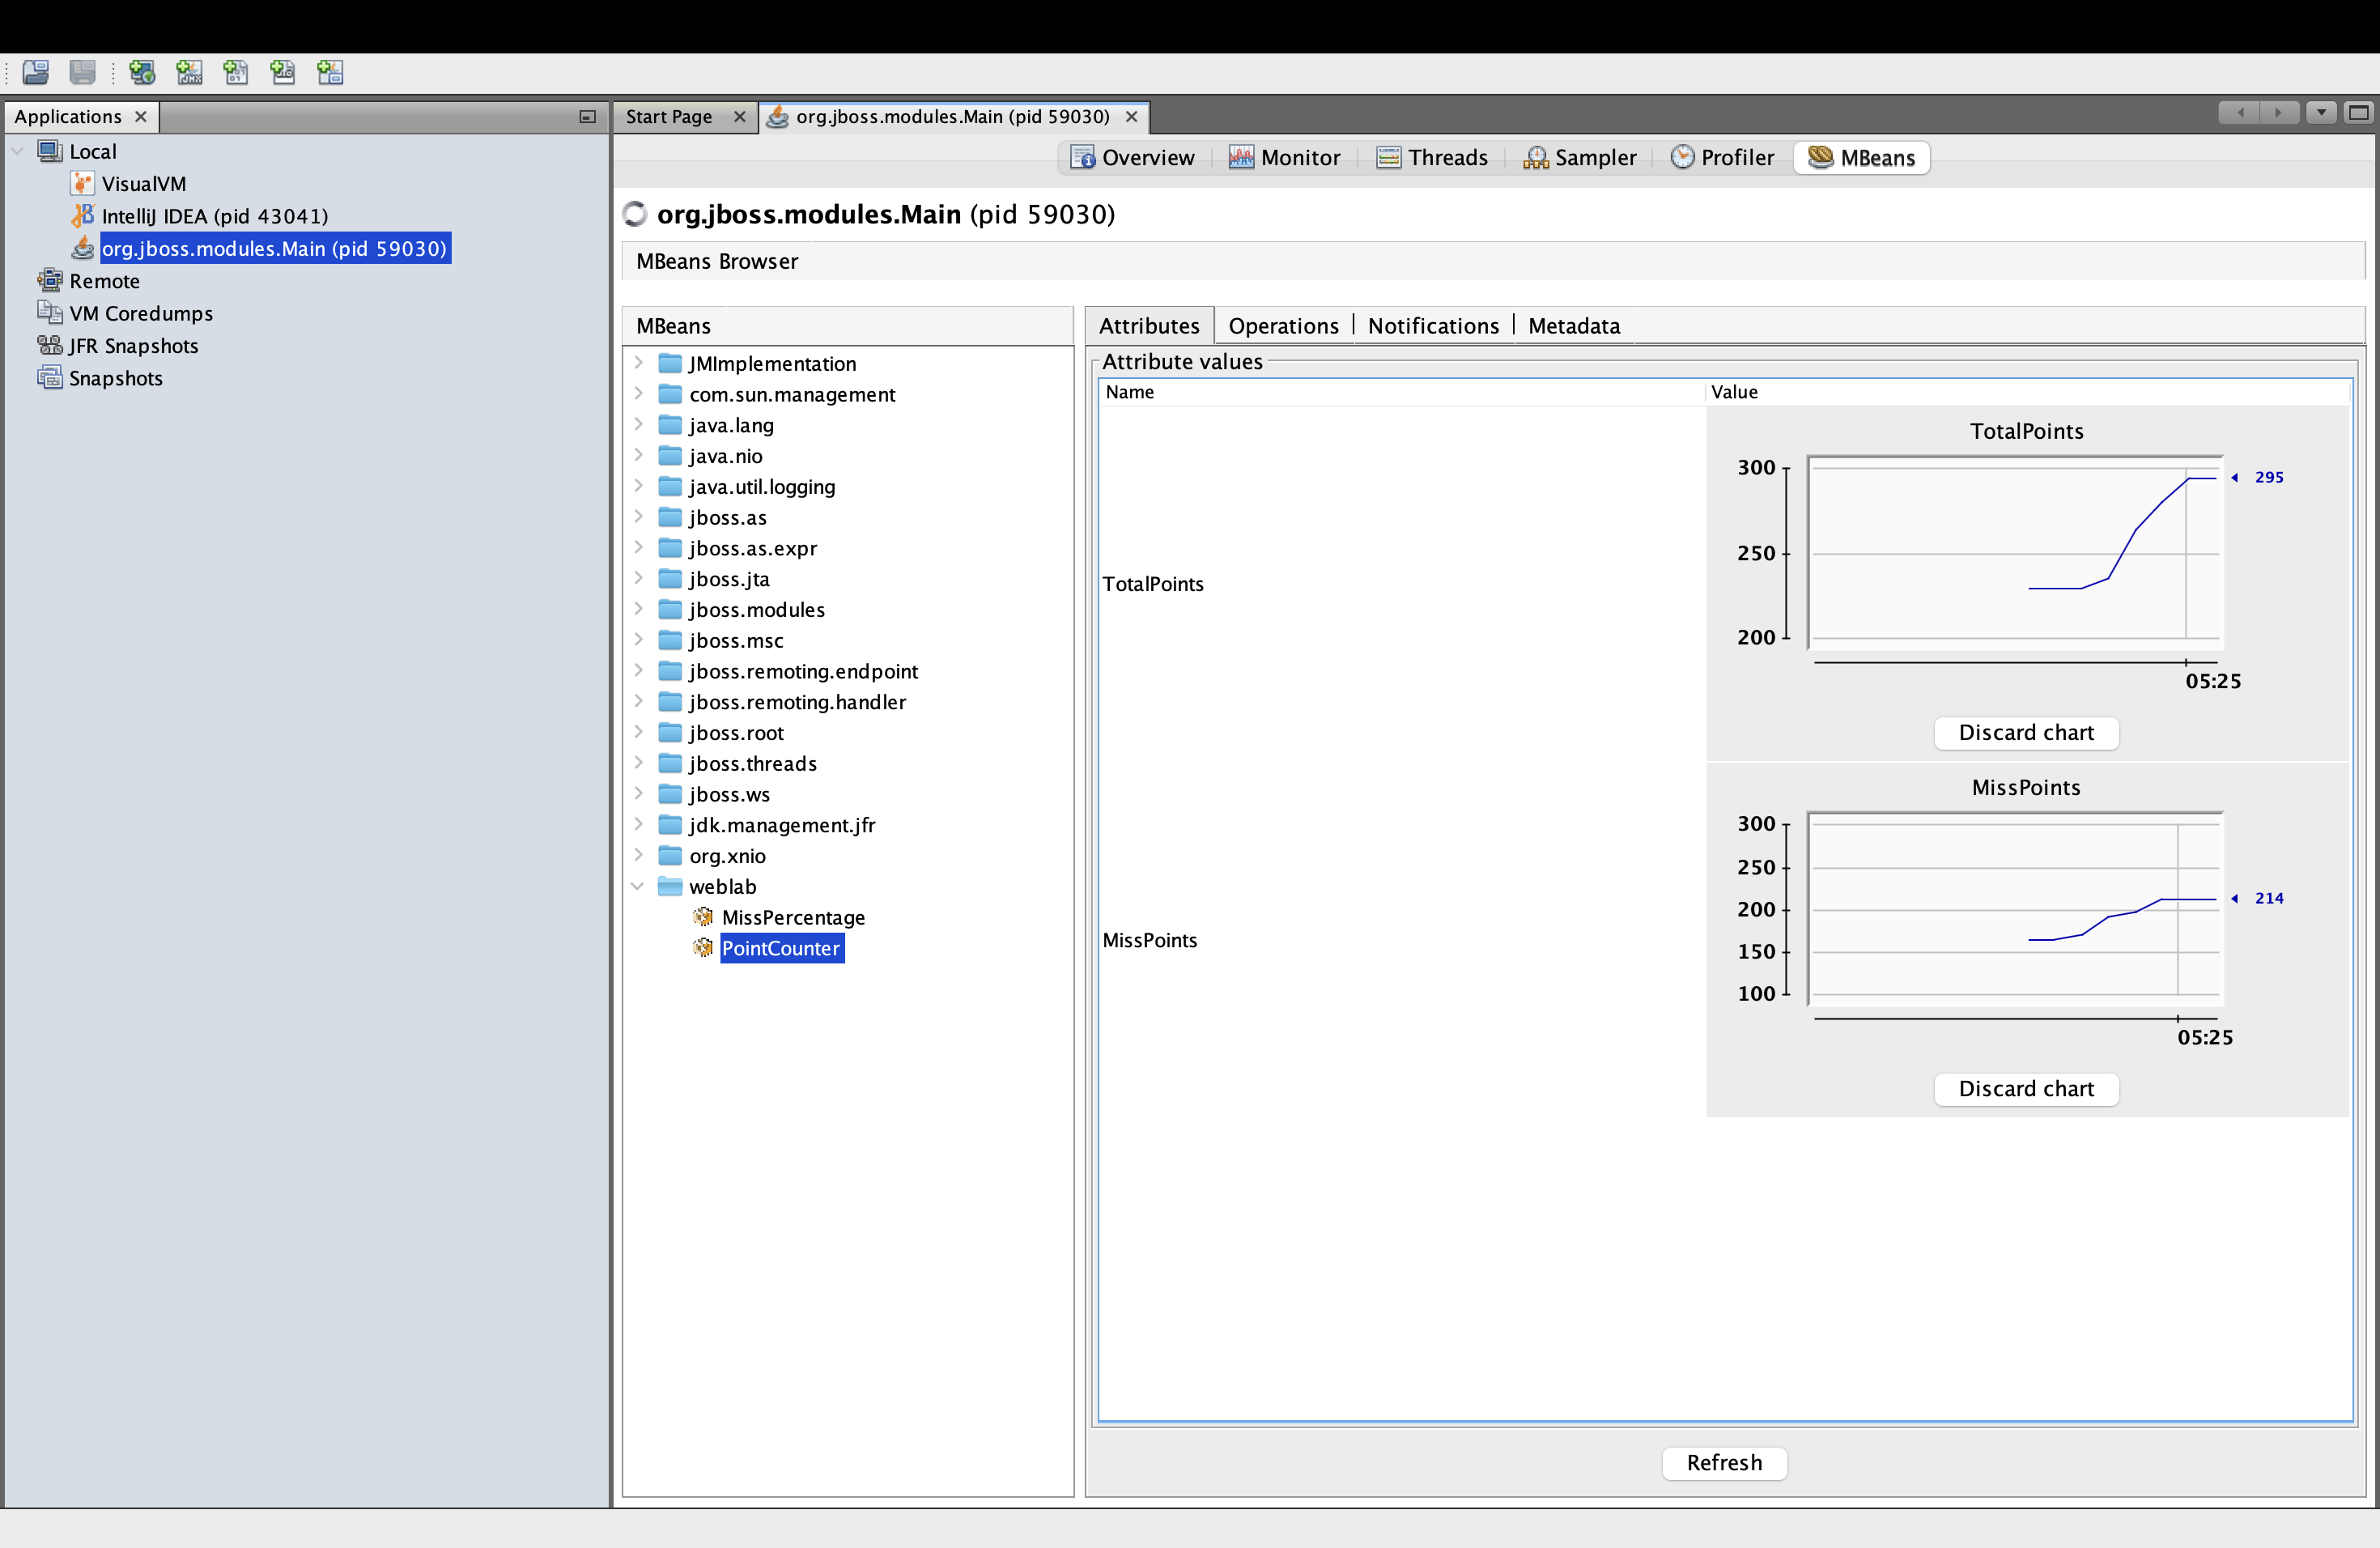
\includegraphics[width=0.7\textwidth]{screenshots/vvm-pointcounter.png}
    \caption{Графики изменения \texttt{TotalPoints} и \texttt{MissPoints} в VisualVM.}
    \label{fig:visualvm-pointcounter}
\end{figure}

На рисунке \ref{fig:visualvm-misspercentage} показан график изменения атрибута \texttt{MissPercentage} MBean \texttt{MissPercentage} с течение времени. 

\begin{figure}[H]
    \centering
    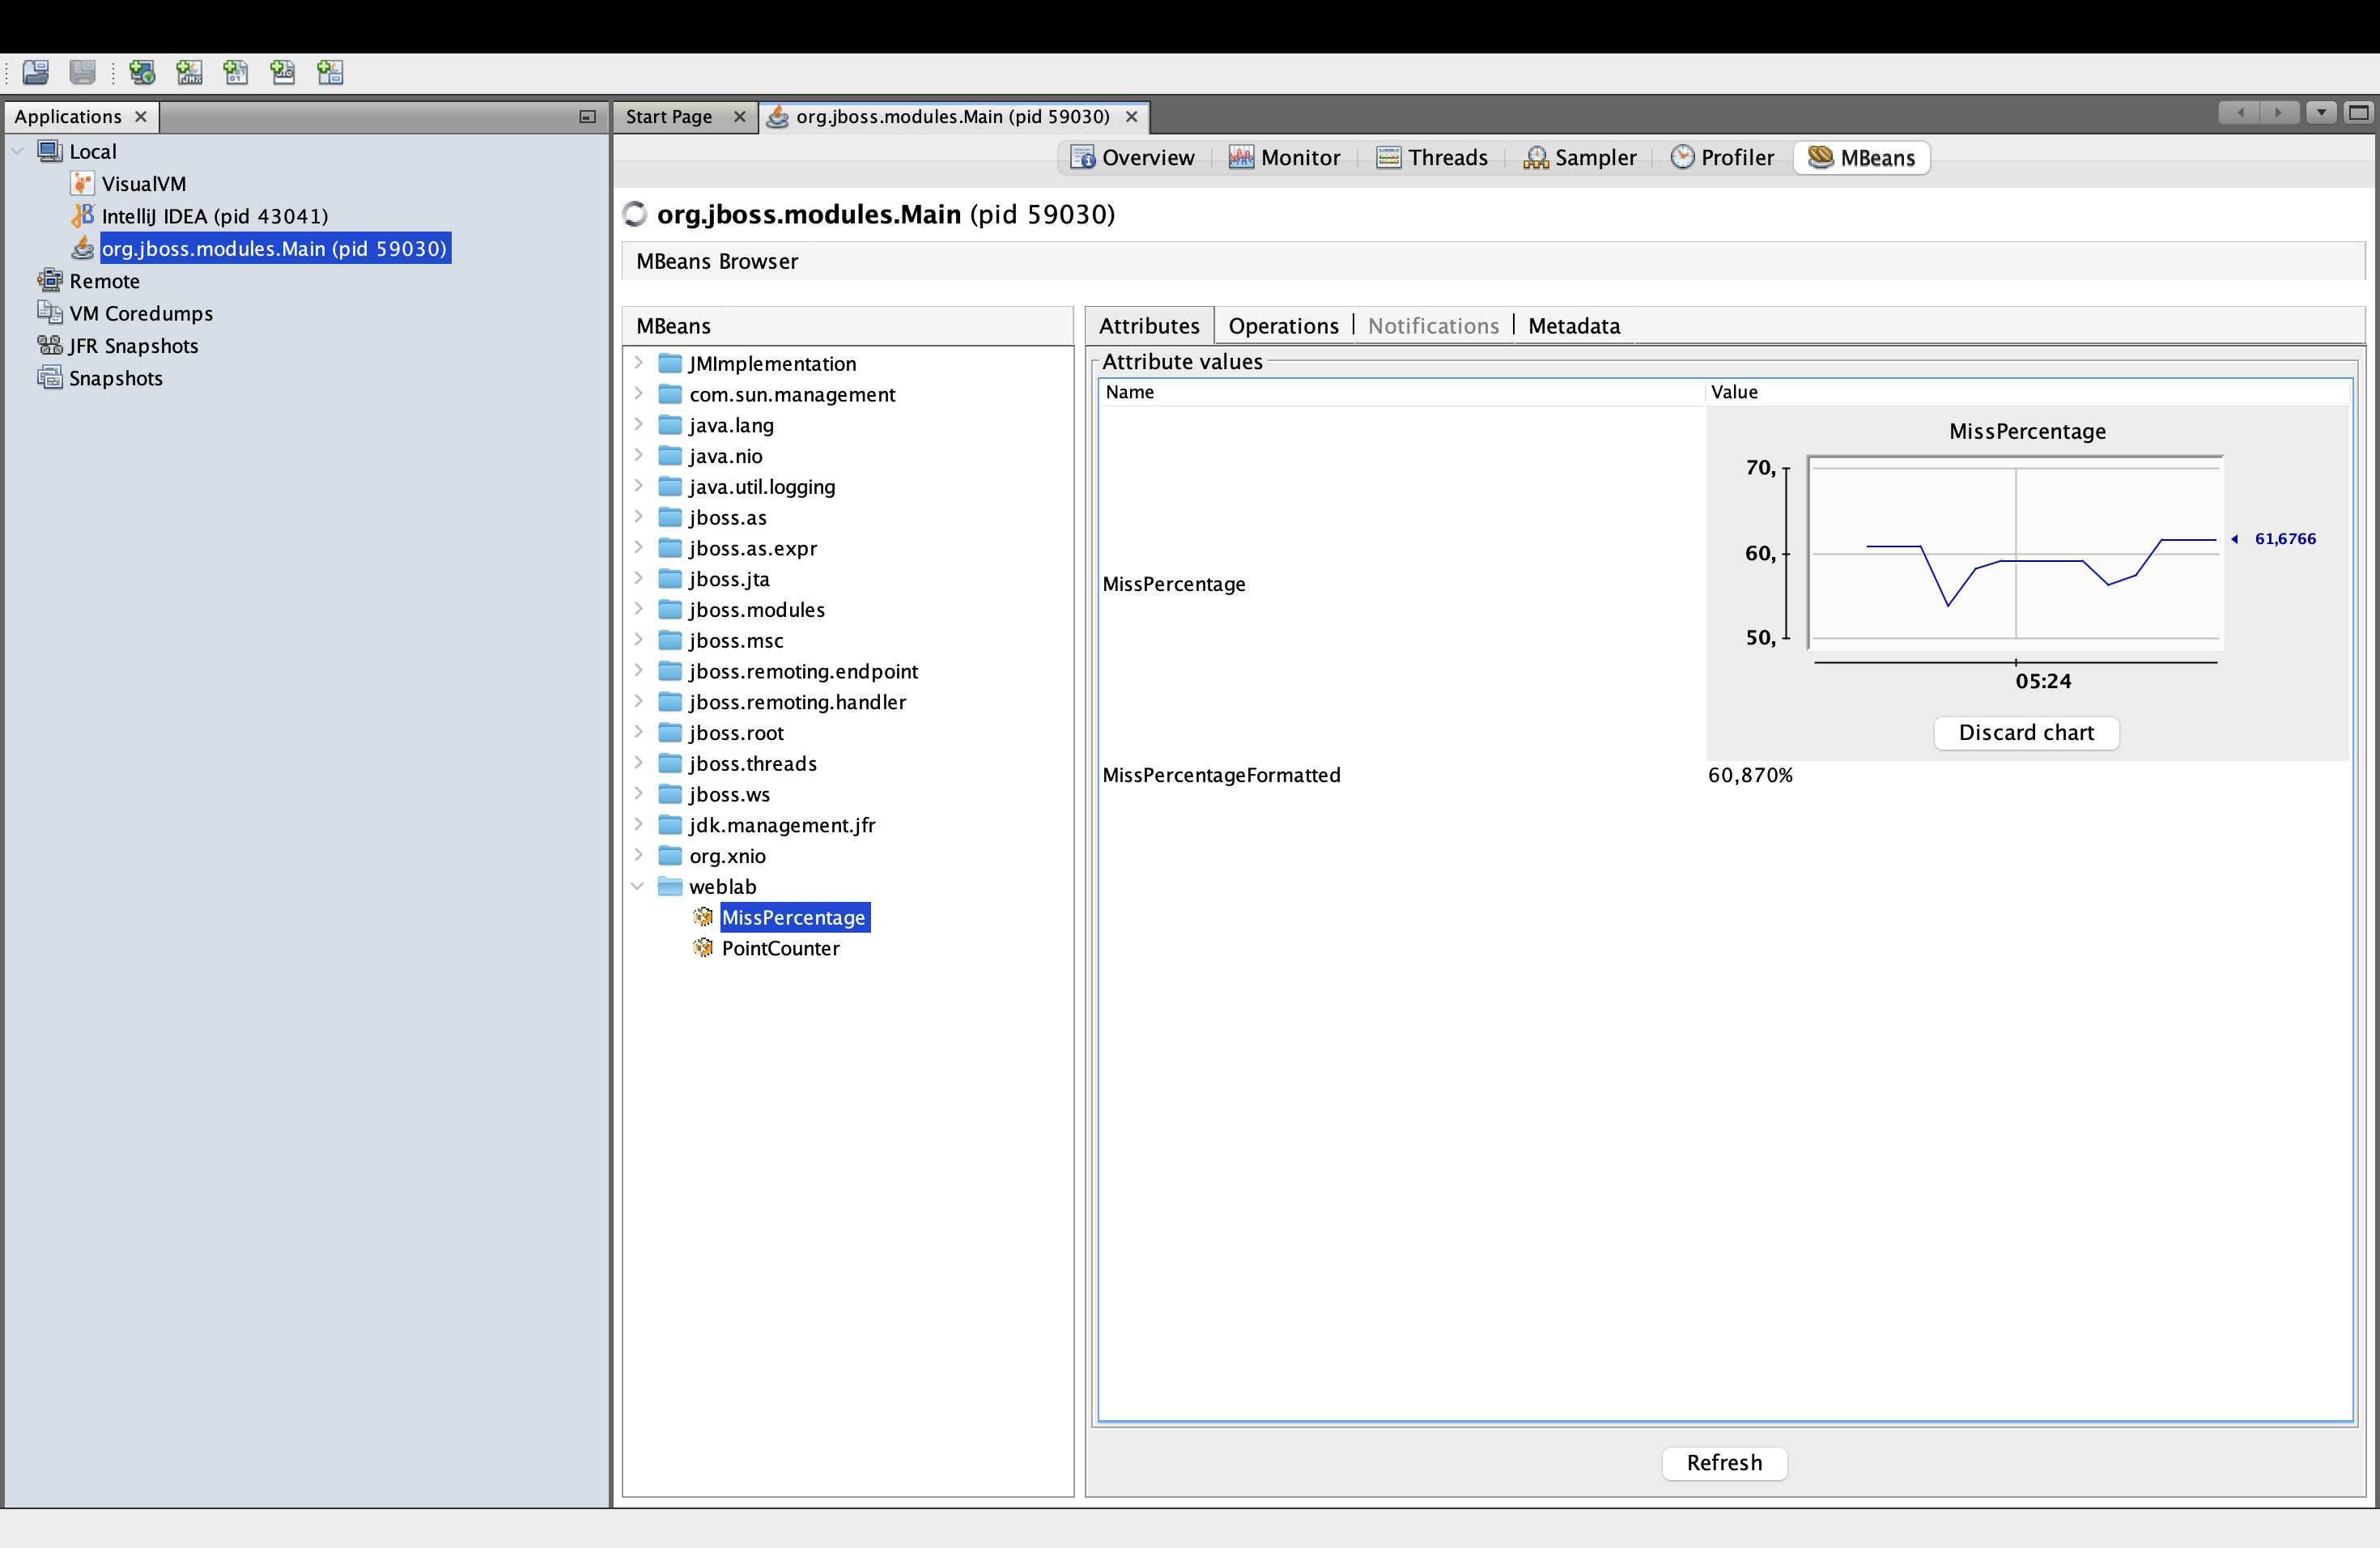
\includegraphics[width=0.7\textwidth]{screenshots/vvm-misspercentage.png}
    \caption{График изменения \texttt{MissPercentage} в VisualVM.}
    \label{fig:visualvm-misspercentage}
\end{figure}

\subsubsection{Анализ использования памяти}

Для определения классов, объекты которых занимают наибольший объём памяти, был запущен профилировщик по памяти для всех классов приложения.

На рисунке \ref{fig:heap-top-classes} представлены классы, объекты которых потребляют наибольший объём памяти JVM.

\begin{figure}[H]
    \centering
    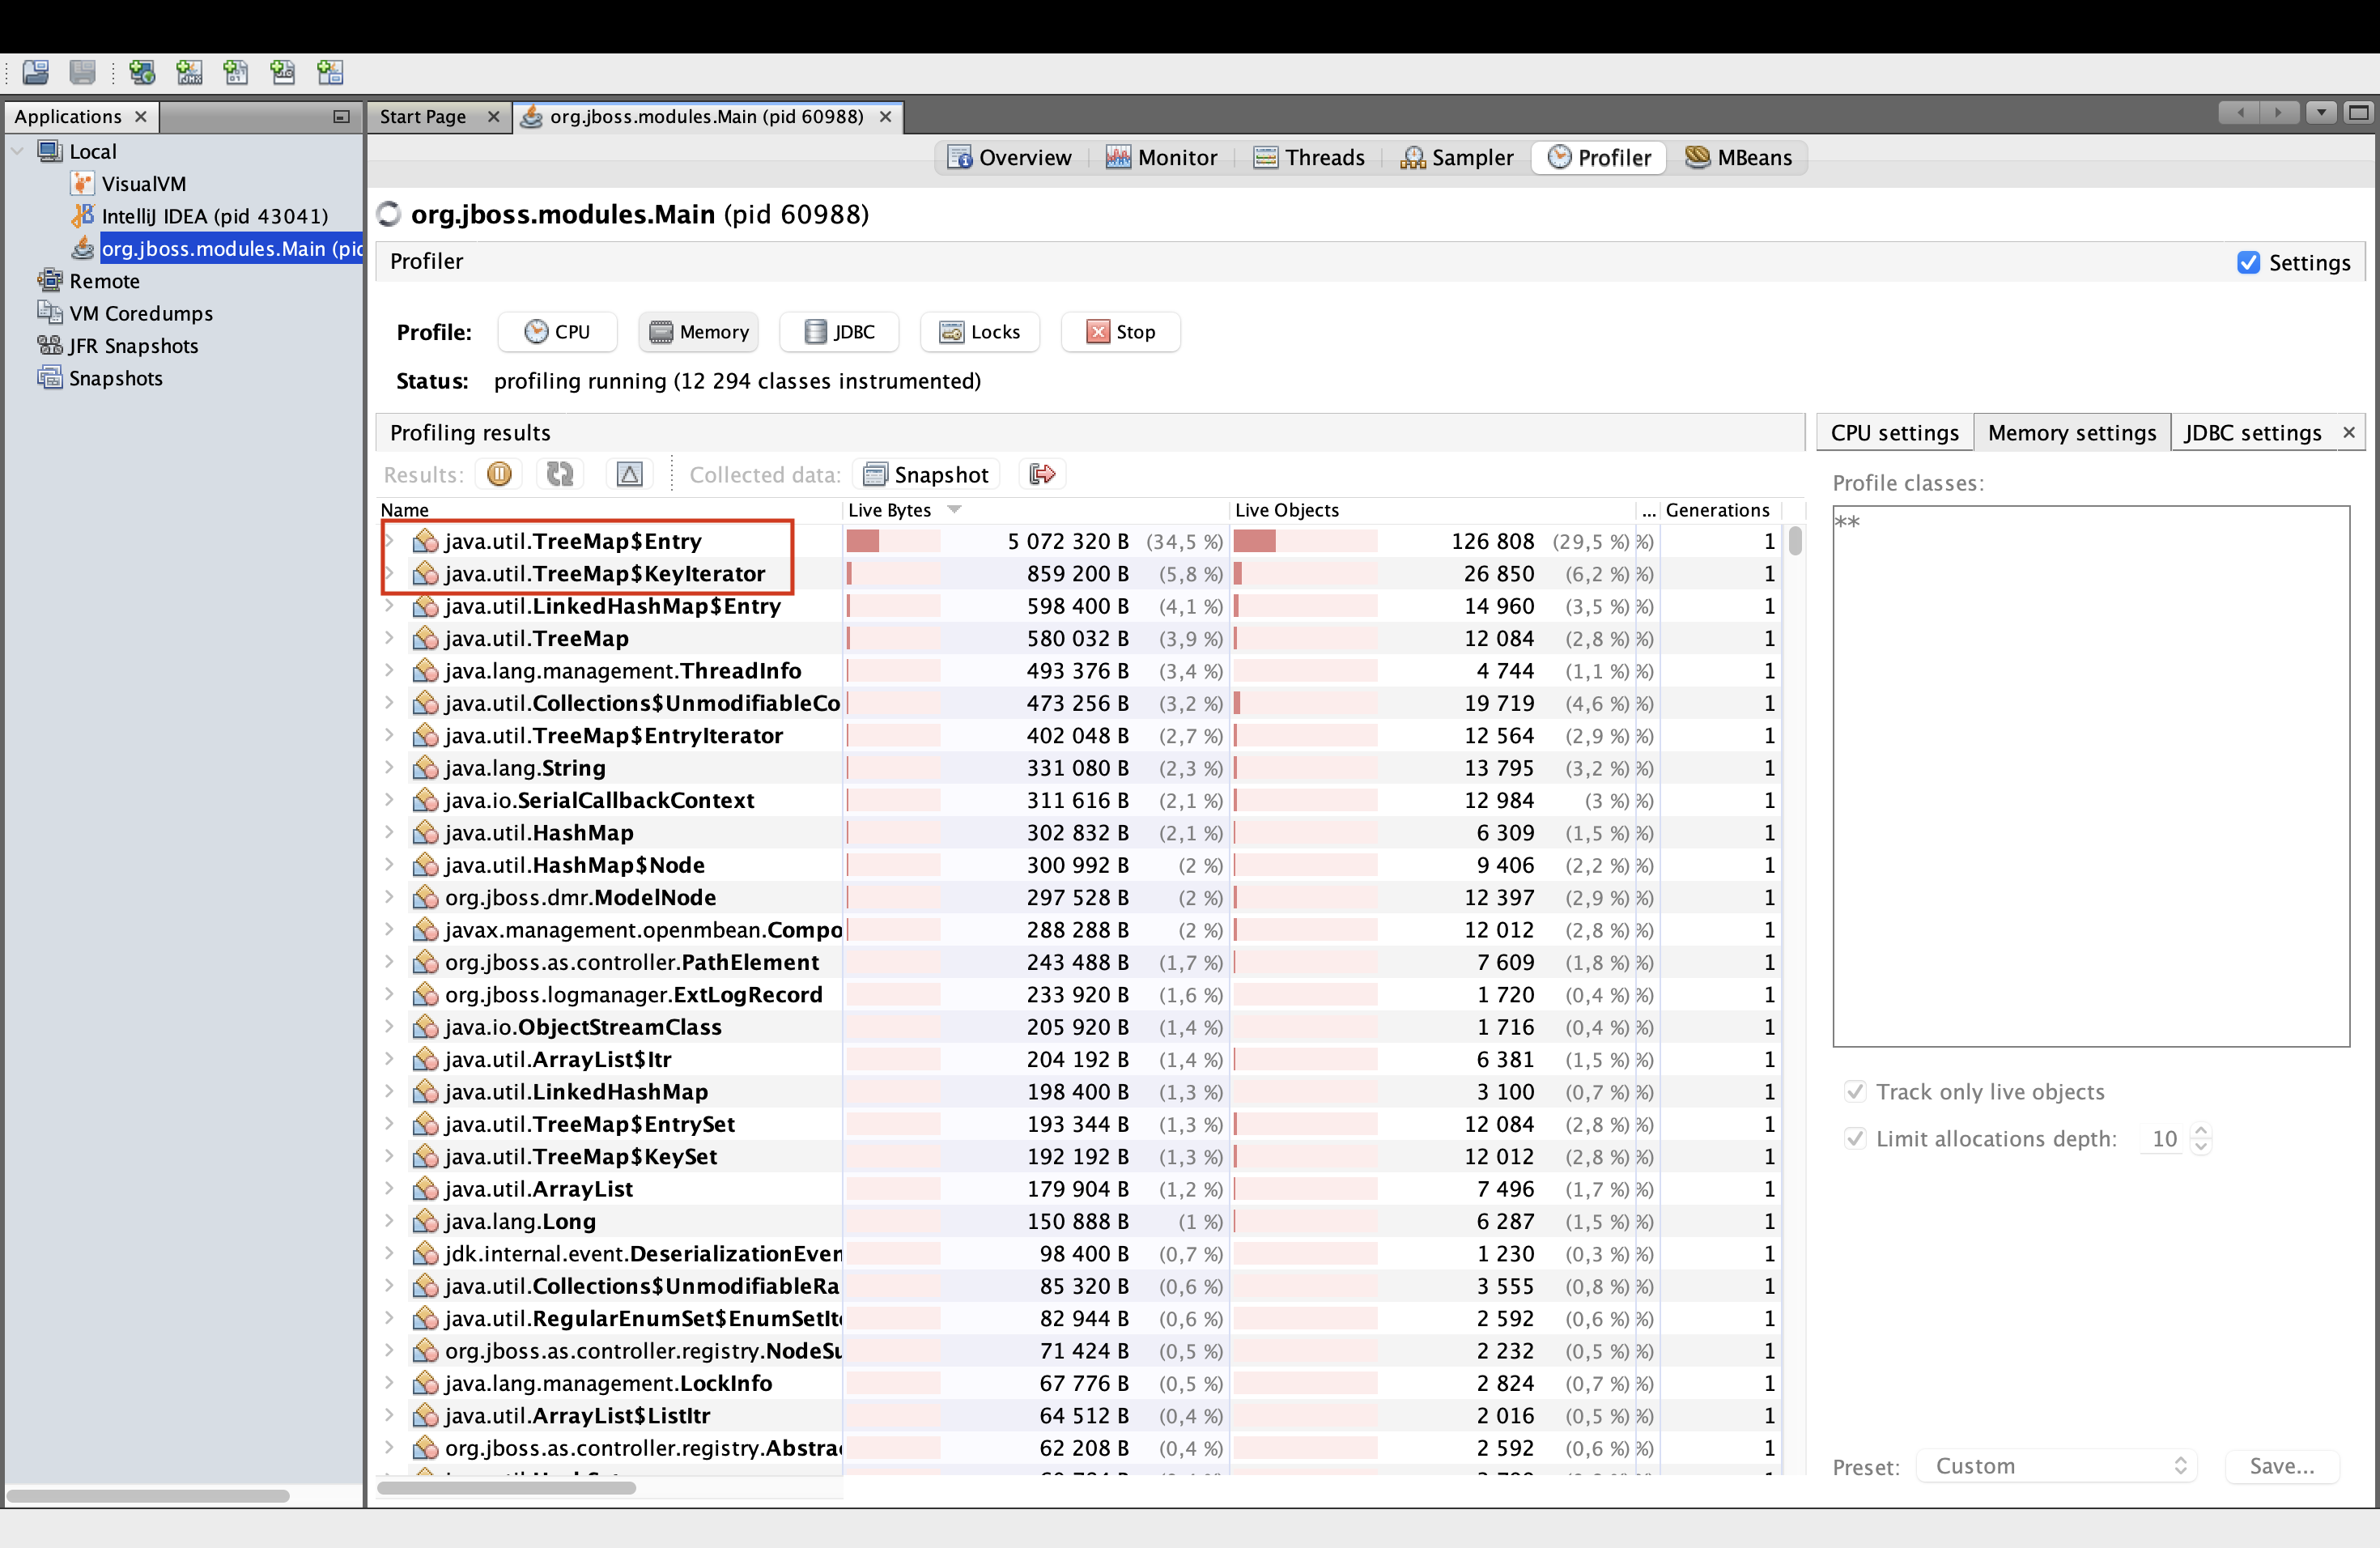
\includegraphics[width=0.7\textwidth]{screenshots/vvm-1.png}
    \caption{Классы с наибольшим объёмом памяти.}
    \label{fig:heap-top-classes}
\end{figure}

Как видно из результатов:
\begin{itemize}
    \item \textbf{java.util.TreeMap\$Entry} занимает \textbf{34.5\%} памяти. Это связано с хранением данных в коллекциях, используемых приложением.
    \item \textbf{java.util.TreeMap\$KeyIterator} занимает \textbf{5.8\%} памяти. Данный класс используется при итерации по элементам коллекций.
\end{itemize}

На рисунке \ref{fig:heap-user-classes} представлены пользовательские классы проекта, отсортированные по объёму занимаемой памяти.

\begin{figure}[H]
    \centering
    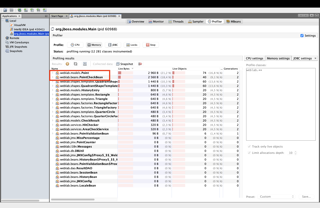
\includegraphics[width=0.7\textwidth]{screenshots/vvm-2.png}
    \caption{Пользовательские классы с наибольшим объёмом памяти.}
    \label{fig:heap-user-classes}
\end{figure}

Результаты анализа:
\begin{itemize}
    \item \textbf{weblab.models.Point} занимает \textbf{21.2\%} памяти среди всех пользовательских объектов. Это объясняется тем, что каждая проверка точки создаёт экземпляр данного класса, а история проверок сохраняется в памяти приложения.
    \item \textbf{weblab.beans.PointCheckBean} занимает \textbf{18.4\%} памяти. Данный бин является \texttt{@RequestScoped} и создаётся для каждого HTTP-запроса, что приводит к накоплению экземпляров при интенсивном использовании приложения.
\end{itemize}